% !TEX root = main.tex
%%%%%%%%%%%%%%%%%%%%%%%%%%%%%%%%%%%%%%%%%%%%%%%%%%%%%%
\section{実験方法および結果}
%%%%%%%%%%%%%%%%%%%%%%%%%%%%%%%%%%%%%%%%%%%%%%%%%%%%%%
 実験装置を図\ref{fig:0deg}の状態から時計回りに90~deg~回転させ,手を離したときの角度推移を観測する.
実験を複数回行い,その平均値の角度推移をグラフにプロットする.また,同時に角速度の推移もプロットし,観測する.
なお,角速度データはノイズが多かったため,csvファイルの角速度データに対して,Pythonのpykalmanライブラリを用いてカルマンフィルタを通し,平滑化している.
時刻tにおけるPWM信号のDuty比$D(t)$は,式(3.7)より,
\begin{equation}
	D(t)=\frac{I(t)}{I_{max}}
\end{equation}
とする.

\begin{figure}[h]
	\centering
	\begin{minipage}{0.3\columnwidth}
	  \centering
	  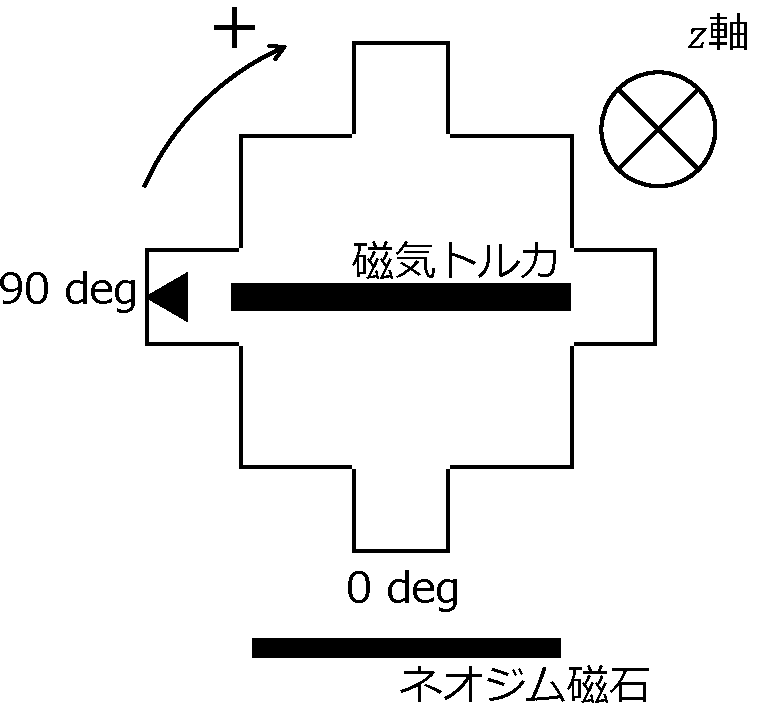
\includegraphics[width=\columnwidth]{./figure/90deg-crop.pdf}
	  \subcaption{角度90~deg}
	  \label{fig:90deg}
	\end{minipage}
	\hspace{5mm}
	\begin{minipage}{0.3\columnwidth}
	  \centering
	  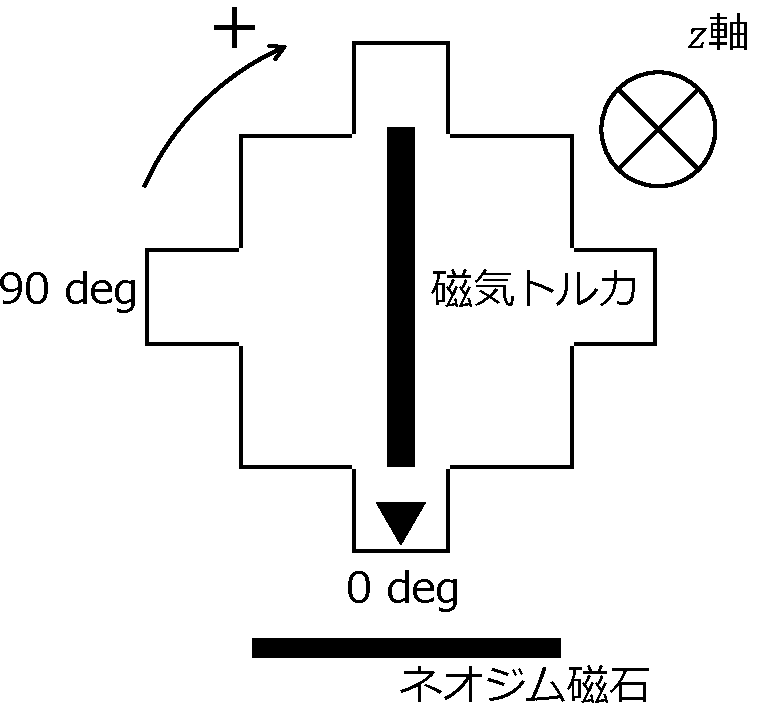
\includegraphics[width=\columnwidth]{./figure/0deg-crop.pdf}
	  \subcaption{角度0~deg}
	  \label{fig:0deg}
	\end{minipage}
	\caption{Duty比50\%としたとき}
	\label{fig:method}
  \end{figure}

 また,ガウスメータを用いて作製した磁気トルカの電圧に対する磁束密度の値を測定した.

\subsection{Duty比100\%・Duty比50\%による制御}
\subsubsection{実験方法}
 PWM信号のDuty比を,50\%と100\%として実験を行う.


\subsubsection{実験結果}
 Duty比を50\%としたときの結果を図\ref{fig:duty50deg},図\ref{fig:duty50degpers}に,100\%としたときの結果を図\ref{fig:duty100deg},図\ref{fig:duty100degpers}に示す.
図に示すようにオーバーシュートが大きく,振動回数が2回となっている.
また,磁気トルカに触ると明らかに発熱していた.
発熱を抑えようとすれば整定時間が伸びる傾向にあった.

\begin{figure}[h]
	\centering
	\begin{minipage}{0.43\columnwidth}
	  \centering
	  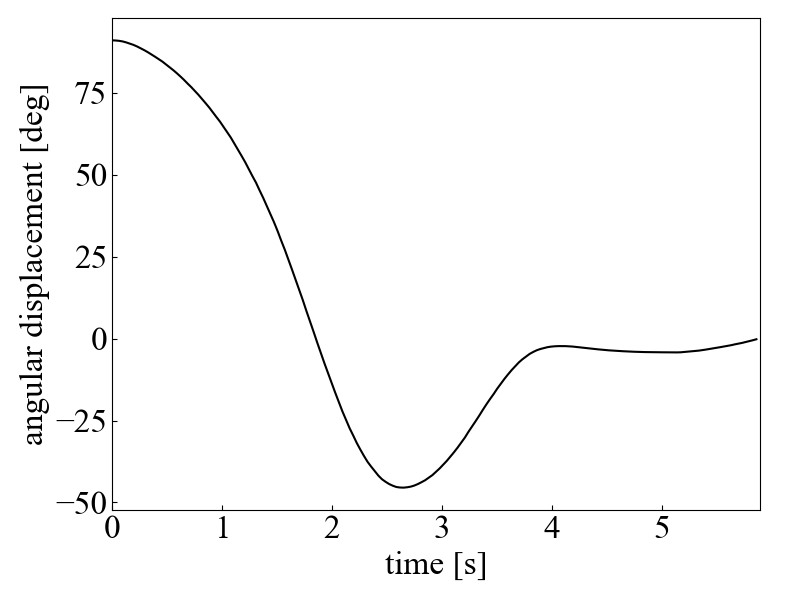
\includegraphics[width=\columnwidth]{./figure/duty50deg.png}
	  \subcaption{角度}
	  \label{fig:duty50deg}
	\end{minipage}
	\hspace{5mm}
	\begin{minipage}{0.43\columnwidth}
	  \centering
	  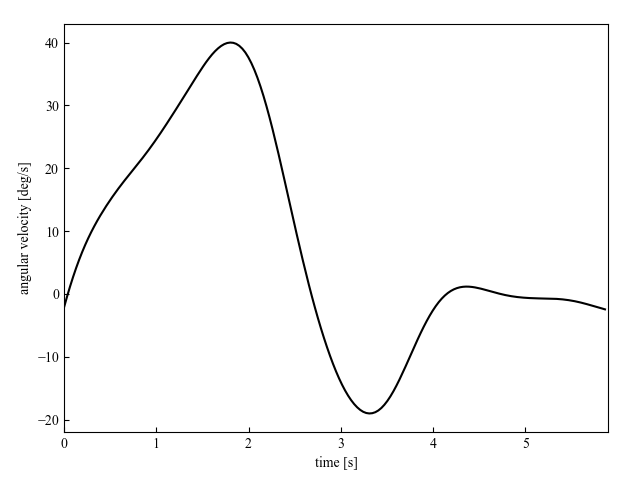
\includegraphics[width=\columnwidth]{./figure/duty50degpers.png}
	  \subcaption{角速度}
	  \label{fig:duty50degpers}
	\end{minipage}
	\caption{PWM信号のDuty比を50\%で連続入力したとき}
  \end{figure}

  \begin{figure}[h]
	\centering
	\begin{minipage}{0.43\columnwidth}
	  \centering
	  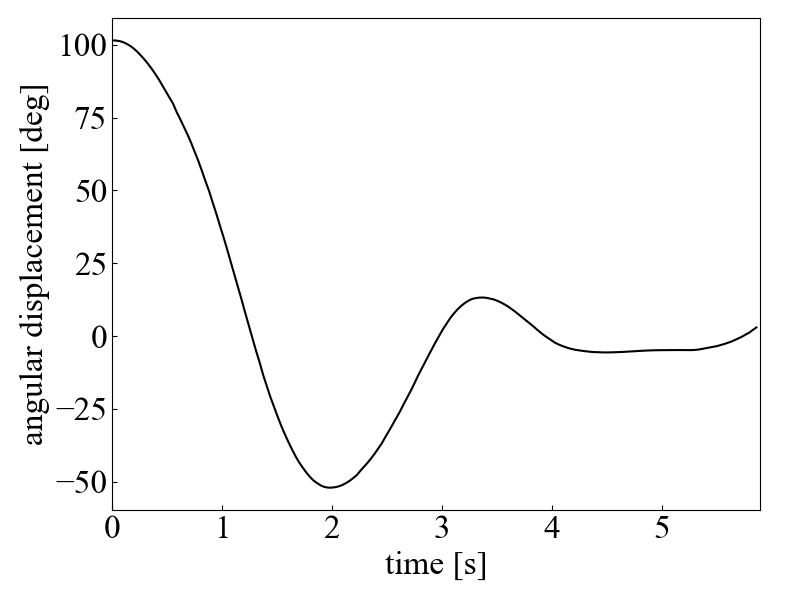
\includegraphics[width=\columnwidth]{./figure/duty100deg.png}
	  \subcaption{角度}
	  \label{fig:duty100deg}
	\end{minipage}
	\hspace{5mm}
	\begin{minipage}{0.43\columnwidth}
	  \centering
	  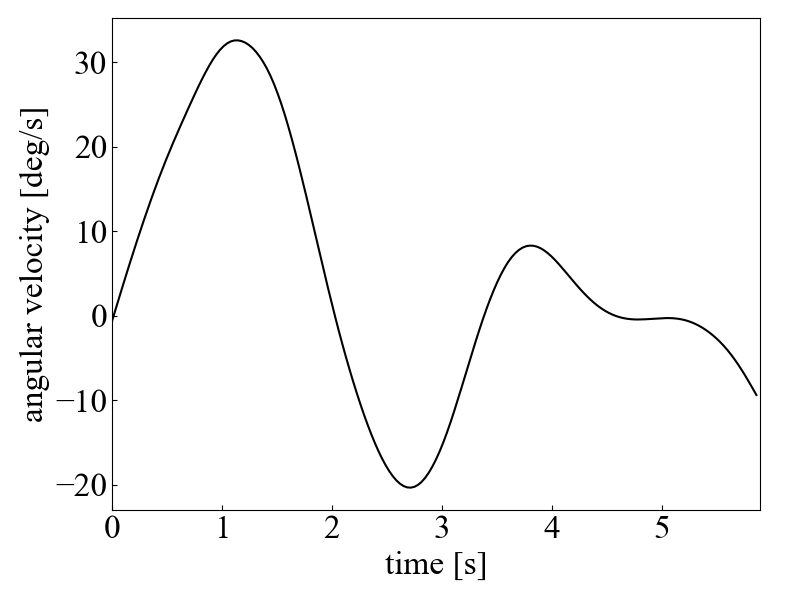
\includegraphics[width=\columnwidth]{./figure/duty100degpers.png}
	  \subcaption{角速度}
	  \label{fig:duty100degpers}
	\end{minipage}
	\caption{PWM信号のDuty比を100\%で連続入力したとき}
  \end{figure}

\subsection{P制御}
\subsubsection{実験方法}
 Pコントローラを$I(t) = k_P |\theta(t)|$とし,実験を行う.

\subsubsection{実験結果}
 何度か実験を行って$k_P$を調整し,$k_P=0.05$としたときの結果を図\ref{fig:Pdeg},図\ref{fig:Pdegpers}に示す.
整定時間は3.8 s ,定常偏差は2.78 deg であった.

\begin{figure}[h]
	\centering
	\begin{minipage}{0.43\columnwidth}
	  \centering
	  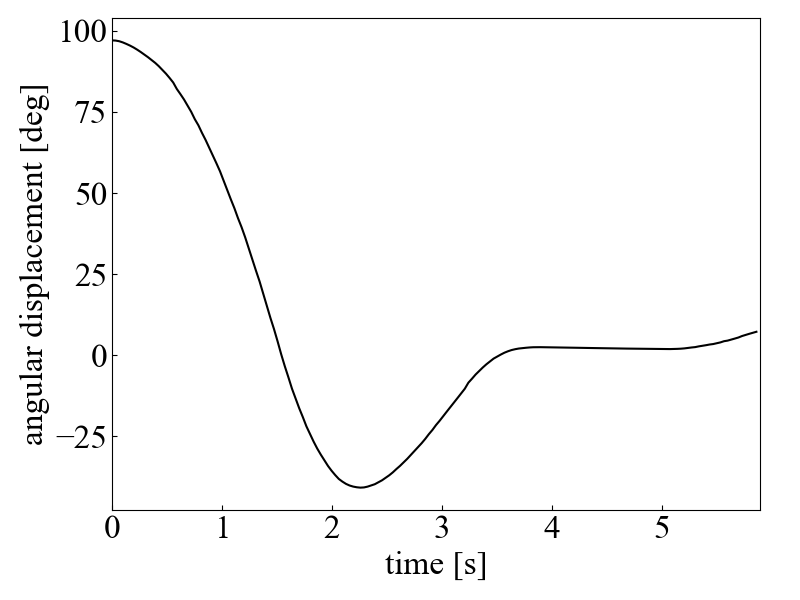
\includegraphics[width=\columnwidth]{./figure/Pdeg.png}
	  \subcaption{角度}
	  \label{fig:Pdeg}
	\end{minipage}
	\hspace{5mm}
	\begin{minipage}{0.43\columnwidth}
	  \centering
	  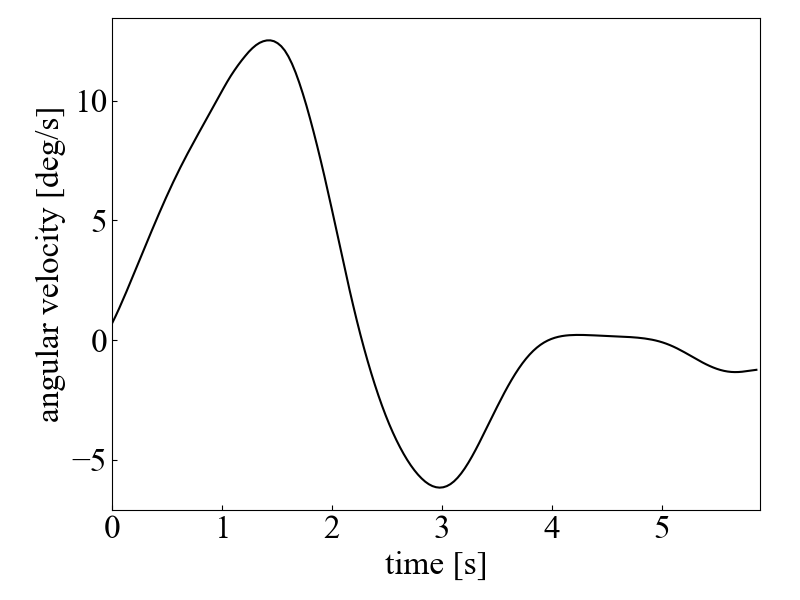
\includegraphics[width=\columnwidth]{./figure/Pdegpers.png}
	  \subcaption{角速度}
	  \label{fig:Pdegpers}
	\end{minipage}
	\caption{コントローラをP制御で設計した場合}
	\label{fig:P}
  \end{figure}

\subsection{PD制御}
\subsubsection{実験方法}
 Pコントローラを$I(t) = k_P |\theta(t)| + k_D|\frac{d\theta(t)}{dt}|$とする.
なお,$\frac{d\theta(t)}{dt}$は,プログラムの1ループ前の角度を$\theta_\mathrm{pre}(t)$とし,$\frac{d\theta(t)}{dt} = \theta(t)-\theta_\mathrm{pre}(t)$で近似する.
ゲインの決定は,限界感度法を用いて行った.
具体的には,比例ゲイン$k_\mathrm{P}$はオーバーシュートが大きくなっていてかつ$k_\mathrm{D}$が大きければ小さく,整定時間が長くかつ$k_\mathrm{D}$が小さければ大きくする.
微分ゲイン$k_\mathrm{D}$は,オーバーシュートが大きくかつ$k_\mathrm{P}$が小さければ大きく,整定時間が長くかつ$k_\mathrm{P}$が大きければ小さくする.
\subsubsection{実験結果}
 何度か実験を行ってゲインを調整し,$k_P=0.03$,$k_P=0.05$としたときの結果を図\ref{fig:PDdeg},図\ref{fig:PDdegpers}に示す.
整定時間は4.0 s ,定常偏差は-21.3 deg であった.
\begin{figure}[h]
	\centering
	\begin{minipage}{0.43\columnwidth}
	  \centering
	  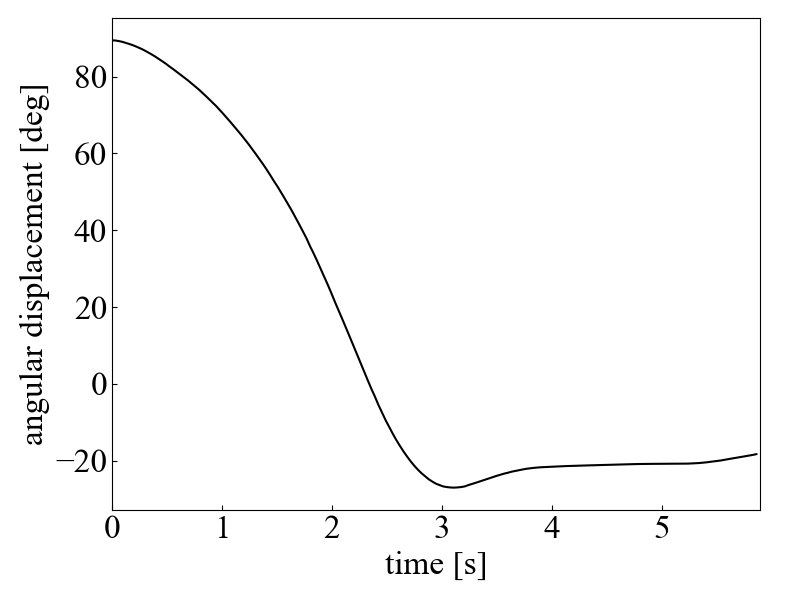
\includegraphics[width=\columnwidth]{./figure/PDdeg.png}
	  \subcaption{角度}
	  \label{fig:PDdeg}
	\end{minipage}
	\hspace{5mm}
	\begin{minipage}{0.43\columnwidth}
	  \centering
	  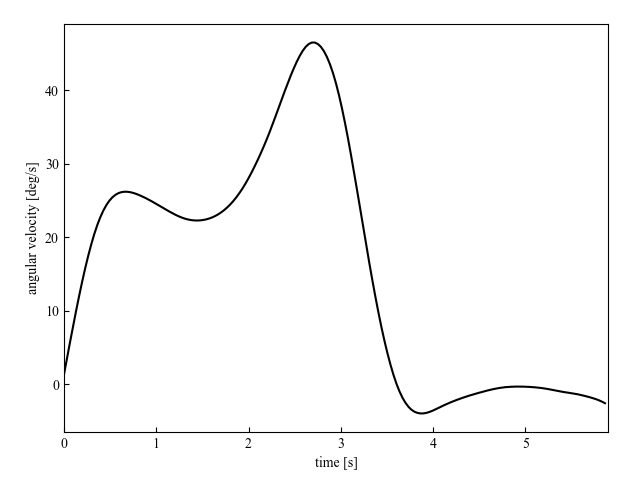
\includegraphics[width=\columnwidth]{./figure/PDdegpers.png}
	  \subcaption{角速度}
	  \label{fig:PDdegpers}
	\end{minipage}
	\caption{コントローラをPD制御で設計した場合}
	\label{fig:PD}
  \end{figure}

\subsection{B-dot制御則}
\subsubsection{実験方法}
 搭載する磁気トルカが1つであるので,目標磁気モーメントは$M=-k_bB_y\omega_z$である.
$|M|=nIS$より,コントローラを$I=\frac{-k_bB_y\omega_z}{nS}$として実験を行う.

\subsubsection{実験結果}
 $k_b=0.02,k_b=0.05,k_b=0.15$としたときの結果を図\ref{fig:bdotdeg},図\ref{fig:bdotdegpers}に示す.
整定時間は3.0 s ,定常偏差は-13.4 deg であった.

\begin{figure}[h]
	\centering
	\begin{minipage}{0.45\columnwidth}
	  \centering
	  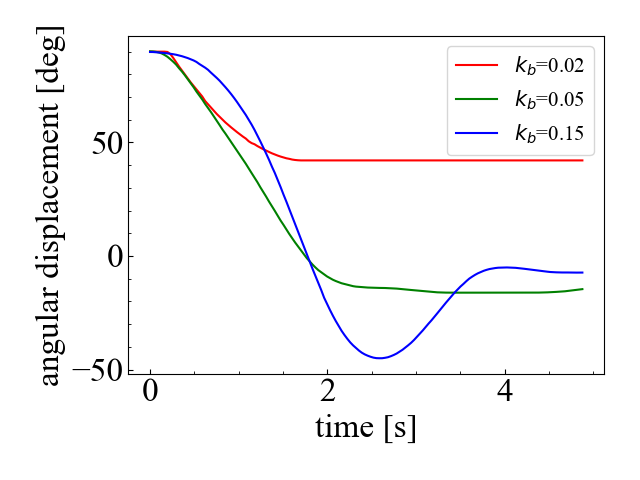
\includegraphics[width=\columnwidth]{./figure/kb5deg.png}
	  \subcaption{角度}
	  \label{fig:bdotdeg}
	\end{minipage}
	\hspace{5mm}
	\begin{minipage}{0.45\columnwidth}
	  \centering
	  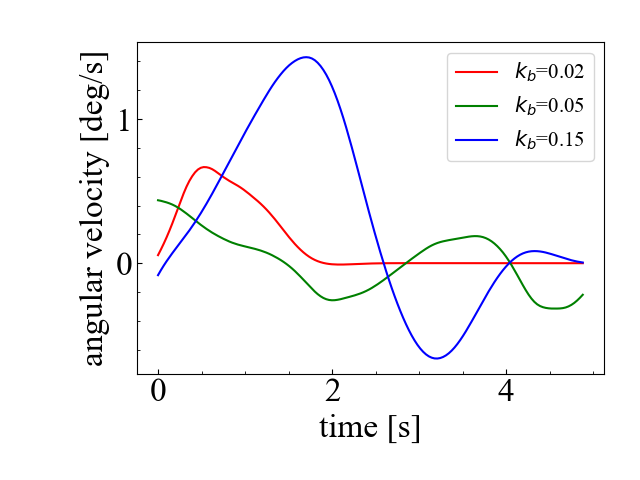
\includegraphics[width=\columnwidth]{./figure/kb5degpers.png}
	  \subcaption{角速度}
	  \label{fig:bdotdegpers}
	\end{minipage}
	\caption{コントローラをB-dot制御則で設計した場合}
	\label{fig:bdot}
\end{figure}


\subsection{クロスプロダクト則}
\subsubsection{実験方法}
 目標磁気モーメントが$M = \frac{K_x c_z + k_x \omega_z}{B_y}$であるので,
コントローラを$I=\frac{K_x c_z + k_x \omega_z}{nSB_y}$として実験を行う.
ゲインの決定は,PD制御と同様に限界感度法に近い操作で.
具体的には,$K$はオーバーシュートが大きくなっていてかつ$k$が大きければ小さく,整定時間が長くかつ$k$が小さければ大きくする.
$k$は,オーバーシュートが大きくかつ$K$が小さければ大きく,整定時間が長くかつ$K$が大きければ小さくする.

\subsubsection{実験結果}
 $K_x=0.04$,$k_x=0.03$としたときの結果を図\ref{fig:crossdeg},図\ref{fig:crossdegpers}に示す.
整定時間は3.8 s ,定常偏差は0.1 deg であった.

\begin{figure}[H]
	\centering
	\begin{minipage}{0.43\columnwidth}
	  \centering
	  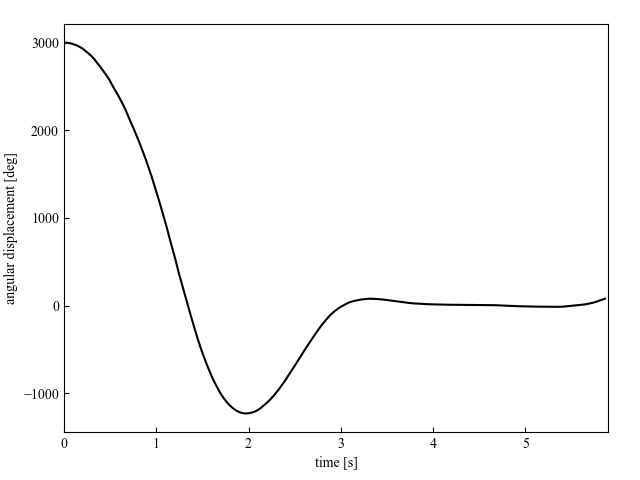
\includegraphics[width=\columnwidth]{./figure/crossdeg.png}
	  \subcaption{角度}
	  \label{fig:crossdeg}
	\end{minipage}
	\hspace{5mm}
	\begin{minipage}{0.43\columnwidth}
	  \centering
	  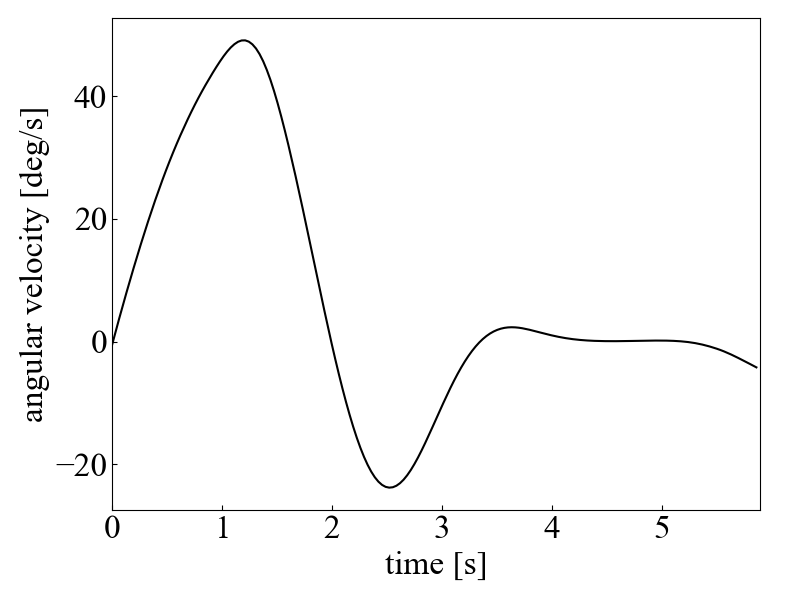
\includegraphics[width=\columnwidth]{./figure/crossdegpers.png}
	  \subcaption{角速度}
	  \label{fig:crossdegpers}
	\end{minipage}
	\caption{コントローラをクロスプロダクト則で設計した場合}
	\label{fig:cross}
\end{figure}

\subsection{考察}
 各結果の整定時間,定常偏差を表\ref{table:result}に示す.
この表から,整定時間に基づいて評価すればB-dot制御則が最適であり,
定常偏差に基づいて評価すればクロスプロダクト則が最も優れた制御則となる結果を得た.
P,PD,クロスプロダクト則は,制御量が角度であるのに対して積分要素を含まないため,ゲインの組み合わせによっては定常偏差が残る.
B-dot制御則は制御量が角速度であるため,定常偏差が残っていると考えられる.
PD制御,クロスプロダクト則については摩擦を考慮して定常偏差,整定時間,オーバーシュートの評価について満足するゲインの設定を行う余地がある.

 3.4節の結果については,測定結果の誤差を考慮すれば,0から15~V~まで比例していると考えることもできるが,
少なからず実験への影響が現れることが考えられる.
\begin{table}[H]
	\centering
	\caption{実験結果}
	\label{table:result}
	\begin{tabular}{|c||c|c|c|c|c|c|}
		\hline
		 & 50\% & 100\% & P制御 & PD制御 & B-dot制御則 & クロスプロダクト則 \\ \hline
		整定時間T [s] & 4.1 & 4.3 & 3.8 & 4.0 & 3.0 & 3.8 \\ \hline
		定常偏差$\theta$ [deg] & -2.4 & -3.9 & 2.78 & -21.3 & -13.4 & 0.1 \\ \hline
	\end{tabular}
\end{table}

 次に,磁気トルカおよび制御理論を検証する実験装置としての評価を行う.
B-dot制御則については,ゲインの調整をしても定常偏差が残りやすく,
角速度を0に指向するというB-dot制御則の特徴が現れていると考えられる.
PD,クロスプロダクト則についてはゲイン設定の余地はあるものの,ゲインの組み合わせにより
オーバーシュートを抑えられたり,整定時間を抑えられたりと,コントローラの設計が行える点から,
人工衛星の姿勢制御についての簡単な実験装置として用いることは可能であると考える.

 本実験装置の宇宙空間との大きな相違点として,発生するトルクの大きさ,転がり軸受に生じる滑り摩擦,空気抵抗が挙げられる.
式(2.1)より,磁気トルカが生み出すトルクは,芯材の透磁率,巻き数,電流値,芯材の断面積および磁束密度に比例していることがわかる.
この中で,本実験装置において宇宙空間と大きく変更した点は,電流値と磁束密度である.
まず電流値については,本研究で用いた用いた磁気トルカは,最大電流値が$I_\mathrm{max}=8.2\times10^2~\mathrm{mA}~$で,実際に用いられているものは,
文献\cite{torquer}においては$130~\mathrm{mA}~$とするものがある.本研究で用いる磁気トルカに流す電流は,常に100\%とは限らないため,最大値の50\%の$4.1\times10^2~\mathrm{mA}~$を用いて計算する.
また地磁気については,本研究で用いたネオジム磁石の,
磁気トルカが反応する距離での磁束密度はおよそ$20~\mathrm{mT}~$であり,日本上空の地磁気は約$30~\mathrm{\mu T}~$である\cite{chijiki}.このことから,
人工衛星で用いられる磁気トルカと,本研究で用いた磁気トルカのトルクについて相対的な比較を行うと,
\begin{equation}
	\frac{20\times10^{-3}~\mathrm{T}}{30\times10^{-6}~\mathrm{T}}\times\frac{410~\mathrm{mA}}{130~\mathrm{mA}} \approx 2000
\end{equation}
となり,この計算からトルクが約2000倍異なることがわかる.
また,宇宙空間は地上とは違い大気がなく,例えばISSの高度での圧力は$10^{-5}~\mathrm{Pa}~$と,地球上($1.013\times10^{5}~\mathrm{Pa}~$)の約$10^{10}$分の1である.
また気体の粘性もほとんどないため,粘性抵抗,圧力抵抗ともに小さく,地上とは大きく異なる点となっている.




\newpage
\section{結論}
\subsection{本研究のまとめ}
 本研究では,人工衛星の模型や実験システムを新規に作製して,磁気トルカによる姿勢制御を検証した.
B-dot制御則については,角速度を0に指向するという,制御理論の特徴が現れる結果となった.
しかし,PD制御・クロスプロダクト則についてはゲイン設定の余地があり,
今回得られた結果から,制御理論としての評価を行うのは尚早と考えられる.\\
 また本研究で作製した実験装置は,転がり軸受の摩擦や外部電源との接続といった部分で宇宙空間の環境とは程遠く,
これを用いて磁気トルカの性能検証やゲイン設定などを行うことはできないと考えられる.
しかし制御理論の一部の特徴(制御量や制御入力による違いなど)を反映できている点はあるため,
そういった特徴を視覚的に理解することができると考える.


\subsection{今後の展望}

 摩擦の影響がない宇宙空間を想定すると,積分要素が含まれていなくても定常偏差は残らない.
転がり軸受の工夫等により摩擦をさらに軽減できれば,PD制御・クロスプロダクト則は定常偏差が残らず,B-dot制御則との役割の違いが現れ,評価が変わる可能性がある. 
そのため本実験装置の改良は,摩擦を減らすことが優先されると考える.
また磁気トルカ駆動用電源の電圧を下げることなどにより,外部電源を実験装置自体に搭載することで,外部電源との接続の影響をなくすことができる.

 今回は磁気トルカを1本のみ用いて検証を行った.しかし実際の人工衛星の姿勢制御では,1軸に対して磁気トルカを2本用いて姿勢制御を行っていることも多いため,
磁気トルカをもう1本増やした検証も必要であると考える.

 実際の人工衛星の挙動や,シミュレーションから得られる角度・角速度推移との定量的な比較ができておらず,
作製した実験装置の有用性の判断ができていない.作製した模型の質量,大きさなどから宇宙空間での挙動のシミュレーションを行い,
その結果との類似点・相違点を比較し,定量的な有用性の判断が必要となる.

 本研究を通して,人工衛星の姿勢制御に関する大まかな知識が得られた.
調査する中で姿勢制御の意義や用いられるアクチュエータとその特徴,目的を知ることができた.
特に磁気トルカを用いた制御理論であるB-dot制御則,クロスプロダクト則について,その設計思想や理論,特性について理解を深めることができた.
今後は,超小型人工衛星について学び,研究し,宇宙利用分野に関して貢献できる人材に成長したいと考えている.